One possible way (out of many) to achieve a cost of $77$ is as follows:

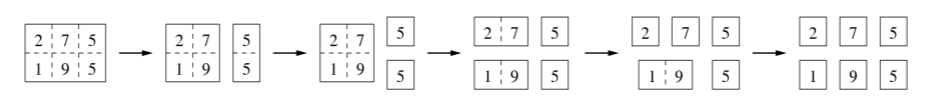
\includegraphics[scale=0.5]{raisins2.png}

The first cut that Bonny asks Peter to make separates the third column from the rest of the chocolate. Bonny needs to pay Peter $29$ raisins for this.

Then Bonny gives Peter the smaller of the two blocks: the one that has two pieces with $5$ raisins each, and asks Peter to cut the block in two in exchange for $10$ raisins.

After this, Bonny gives Peter the largest remaining block: the one having pieces with $2$, $7$, $1$ and $9$ raisins respectively. Bonny asks Peter to cut it horizontally, separating the first and the second row and pays him $19$ raisins.

Following this, Bonny gives Peter the top-left block, paying $9$ raisins. Finally, Bonny asks Peter to split the bottom-left block, paying $10$ raisins.

The total cost to Bonny is $29 + 10 + 19 + 9 + 10 = 77$ raisins. No other cutting arrangement can get the chocolate cut into its $6$ pieces at a smaller cost. 